\documentclass[border=0.2cm]{standalone}
 
% Required package and libraries
\usepackage{tikz}
\usetikzlibrary{patterns.meta,decorations.pathmorphing,patterns}
 
\begin{document}

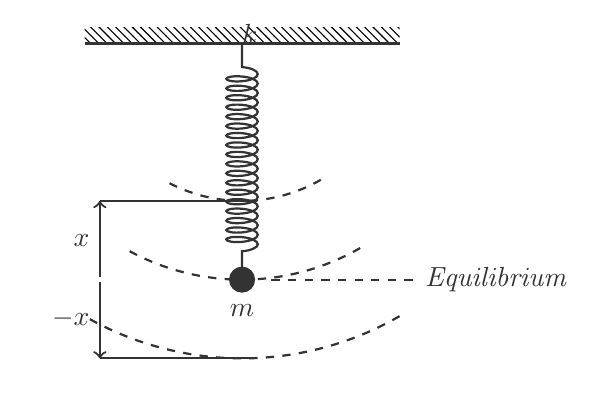
\begin{tikzpicture}[black!80,thick]

% Supporting structure
\fill [pattern = north west lines] (-2,0) rectangle ++(4,0.2);

\draw[thick] (-2,0) -- ++(4,0);
 
% Bob's equilibrium trajectory
\draw[dashed] (-60:3) arc(-60:-120:3);
 
% Bob's minor trajectory
\draw[dashed] (-60:2) arc(-60:-120:2);

% Bob's major trajectory
\draw[dashed] (-60:4) arc(-60:-120:4);

% Spring 
\draw
[
    decoration={
        coil,
        aspect=0.3, 
        segment length=1.2mm, 
        amplitude=2mm, 
        pre length=3mm,
        post length=3mm},
    decorate
] (0,0) -- (-90:3)

% Mass
node[fill,circle,label=south:$m$](m){};
node[midway,right=0.25cm,black]{$k$};

%Arrow-ed change
\draw[] (m.center-|0,0) ++ (0,1) -- ++ (-2,0) 
    edge[<-,edge label'=$x$,shorten >=1pt] (m.center-|-2,0)
  (m.center-|0,0) ++ (0,-1) -- ++ (-2,0) 
    edge[<-,edge label=$-x$,shorten >=1pt] (m.center-|-2,0)
    (m.east) edge[dashed] (m.east-|2,0) 
     (m.east-|2,0) node[right] {\textit{Equilibrium}};

\end{tikzpicture}

\end{document}

